%!TEX program = lualatex -shell-escape
\documentclass{beamer}
\mode<presentation> {
    \usetheme{Marburg}
}
\usepackage[english]{babel}
\usepackage[style=english]{csquotes}
\usepackage{fontspec}
\usepackage{csquotes}
\usepackage{amsmath}
\usepackage{float}
\usepackage{graphicx} % Allows including images
\usepackage{booktabs} % Allows the use of \toprule, \midrule and \bottomrule in tables
\usepackage{makecell}
\usepackage{hyperref}
\usepackage{minted}
\usepackage{caption}
\captionsetup{font=scriptsize}
% TikZ configuration
\usepackage{tikz}
\usetikzlibrary{
    arrows,
    shapes,
    positioning,
    shadows,
    trees,
    calc
}

% Define TikZ elements and styles
\tikzstyle{block} = [rectangle, draw, fill=blue!20,
    text centered, rounded corners, minimum height=2em]
\tikzstyle{line} = [draw, -latex']
\tikzstyle{cloud} = [draw, ellipse,fill=red!20, node distance=3cm,
    minimum height=2em]
\tikzset{
    plain/.style = {
        draw=none,
        fill=none
    }
}

% Biber configuration
\usepackage[
backend=biber,
style=alphabetic,
citestyle=authoryear,
natbib
]{biblatex}

% Configure section slides insertion
\AtBeginSection[]{
  \begin{frame}
  \vfill
  \centering
  \begin{beamercolorbox}[sep=8pt,center,shadow=true,rounded=true]{title}
    \usebeamerfont{title}\insertsection\par%
  \end{beamercolorbox}
  \vfill
  \end{frame}
}

% Footnote without number
\newcommand\blfootnote[1]{%
  \begingroup
  \renewcommand\thefootnote{}\footnote{#1}%
  \addtocounter{footnote}{-1}%
  \endgroup
}


%%% BIBLIOGRAPHY FILE %%%%%%%%%%%%%%%%%%%%%%%%%%%%%%%%%%%%%%%%%%%%%%%%%%%%%%%%%
\addbibresource{literature.bib}

%%% CONTENT %%%%%%%%%%%%%%%%%%%%%%%%%%%%%%%%%%%%%%%%%%%%%%%%%%%%%%%%%%%%%%%%%%%
\begin{document}
%%% TITLE AND AUTHORS %%%%%%%%%%%%%%%%%%%%%%%%%%%%%%%%%%%%%%%%%%%%%%%%%%%%%%%%%
\title[Introduction \& syllabus]{
    Introduction and syllabus \\
    \small{}
}
\author[]{Szymon Talaga and Mikołaj Biesaga} % Your name
\institute[ISS UW]{
    The Robert Zajonc Institute for Social Studies \\ University of Warsaw \\
    \medskip
    \textcolor{blue}{\href{mailto:stalaga@uw.edu.pl}{stalaga@uw.edu.pl}} \\
    \textcolor{blue}{\href{mailto:m.biesaga@uw.edu.pl}{m.biesaga@uw.edu.pl}}
}
\date{2 October 2019} % Date, can be changed to a custom date

%%% SLIDES %%%%%%%%%%%%%%%%%%%%%%%%%%%%%%%%%%%%%%%%%%%%%%%%%%%%%%%%%%%%%%%%%%%%
\frame{\titlepage}

\part[Syllabus]{Syllabus}
\frame{\partpage}

\section[Rules]{Rules of Engagement}
\subsection[Communication]{Communication}
\begin{frame}
    \frametitle{Office Hours, Emails, and Slack}
    \begin{description}[Office Hours:]
        \item[Office Hours:] write us an email or on Slack before coming
        \item[Emails:] the official info will go thorough emails
        \item[Slack:] register at \textcolor{blue}{\href{www.slack.com}{www.slack.com}}
        \item[Google Drive:] materials and presentations will be posted at \textcolor{blue}{\href{https://drive.google.com/a/uw.edu.pl/file/d/1VotLZIEmp4lXnT-NdR0yZ5DDal59FfkI/view?usp=sharing}{Google Drive}}
    \end{description}
    \action<visible@+>{\alert{We will try to answer your inquires as soon as possible but do not count on imidiate response, especially before the deadlines.}}
\end{frame}

\subsection[Workflow]{Workflow}
\begin{frame}
    \frametitle{Workflow}
    \begin{enumerate}
        \item Presentation of basic concepts in real-life examples in the classroom.
        \item Exercises in the classroom.
        \item Home assignments requiring modifying the work done in the classroom.
        \end{enumerate}
        \action<visible@+>{\alert{If you cannot find the answer on Internet you are asking the wrong question.}}
    \end{frame}

\begin{frame}
    \frametitle{Stack Overflow}
    \begin{overprint}
        \onslide<+>
            \begin{figure}
                \centering
                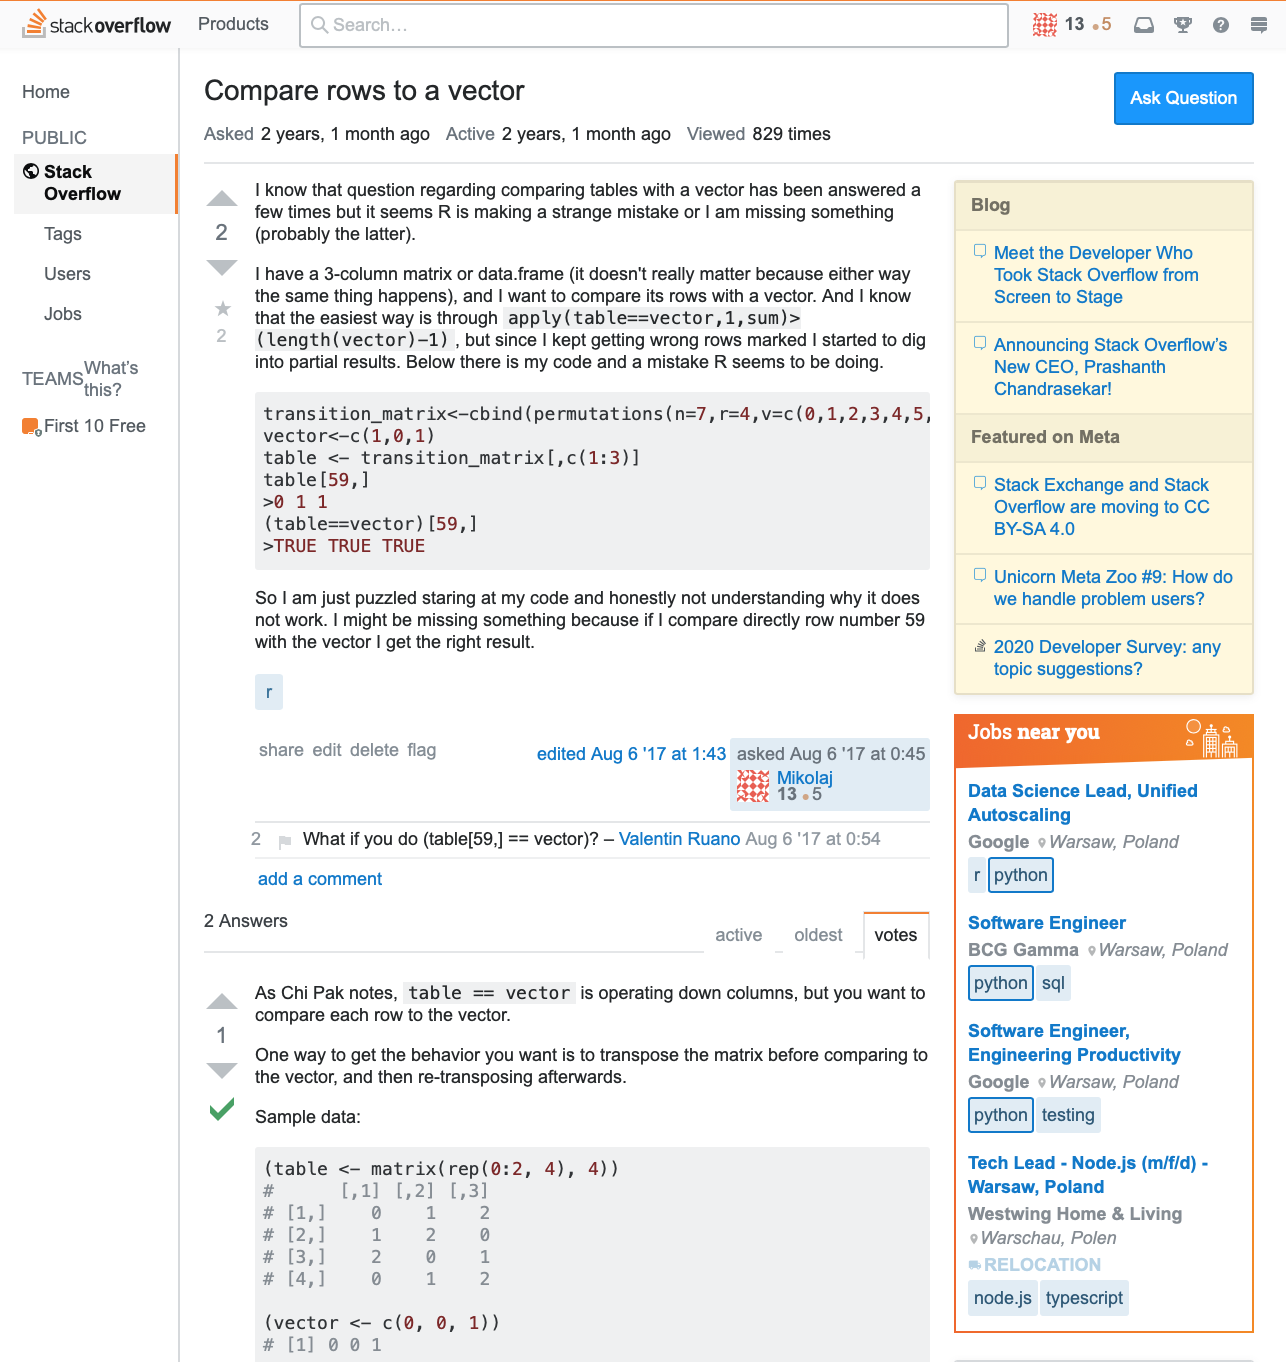
\includegraphics[scale = .3]{png/stack_overflow.png}
            \end{figure}
        \onslide<+>
            \begin{figure}
                \centering
                
\includegraphics[scale = .175]{png/copy_paste.png}
                \caption{from \textcolor{blue}{\href{https://xgohorse.com}{https://xgohorse.com}}}
            \end{figure}
    \end{overprint}
\end{frame}

\subsection[Assessment]{Assessment Criteria}
\begin{frame}
    \frametitle{Assessment Criteria}
    \begin{block}{}
        Final Grade = 30\%$\times$Homeworks + 35\%$\times$Final Exam + 35\%$\times$written report\\
    \end{block}
        \begin{itemize}
        \item Homeworks - 3 written assignments (approximately after weeks 7, 9, and 13)
        \item Final Exam - will cover theoretical material discussed in the classroom (15.01.2019)
        \item Written Report - a research project proposal formulating a research problem that can be addressed with the methods discussed during the course (due to the last class - 22.01.2019)
    \end{itemize}
\end{frame}

\subsection[Attendance]{Attendance}
\begin{frame}
    \frametitle{Attendance}
    \begin{itemize}
        \item You are allowed to miss up to 2 classes without formal excuse
        \item  absence does not exempt from doing homework assignments
    \end{itemize}
    \action<visible@+>{\alert{It is better not to miss classes because this is a relatively challenging course and it will be hard to cover the material from the class at home.}}
\end{frame}


\part[Introduction]{Introduction}
\frame{\partpage}

\section[CSS]{Computational Social Science}

\begin{frame}
    \frametitle{What is Computational Social Science?}
    \begin{definition}{}
        In the most general sense \emph{Computational Social Science} is a data-driven approach which uses computational methods in studying social phenomena.
    \end{definition}
    \begin{definition}{}
        \emph{Data Science} on the other hand is a broader term than Computational Social Science. It describes the theory and practice of extracting knowledge and insight from data.
    \end{definition}
\end{frame}

\begin{frame}{General interest in data science}
    \begin{figure}
    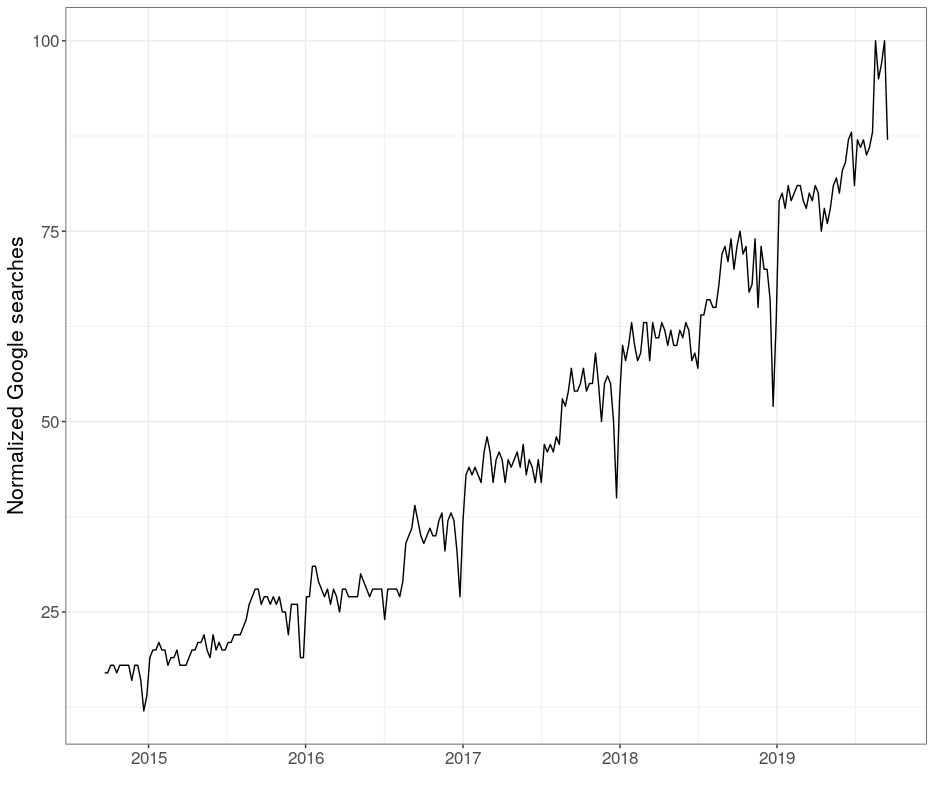
\includegraphics[width = .8\framewidth]{png/ds-searches.png}
    \caption{Growth of "data science" Google search}
    \end{figure}
\end{frame}

\subsection{Research Methods}

\begin{frame}
    \frametitle{Traditional Research Methods}
        \only<0>{
            \begin{figure}
                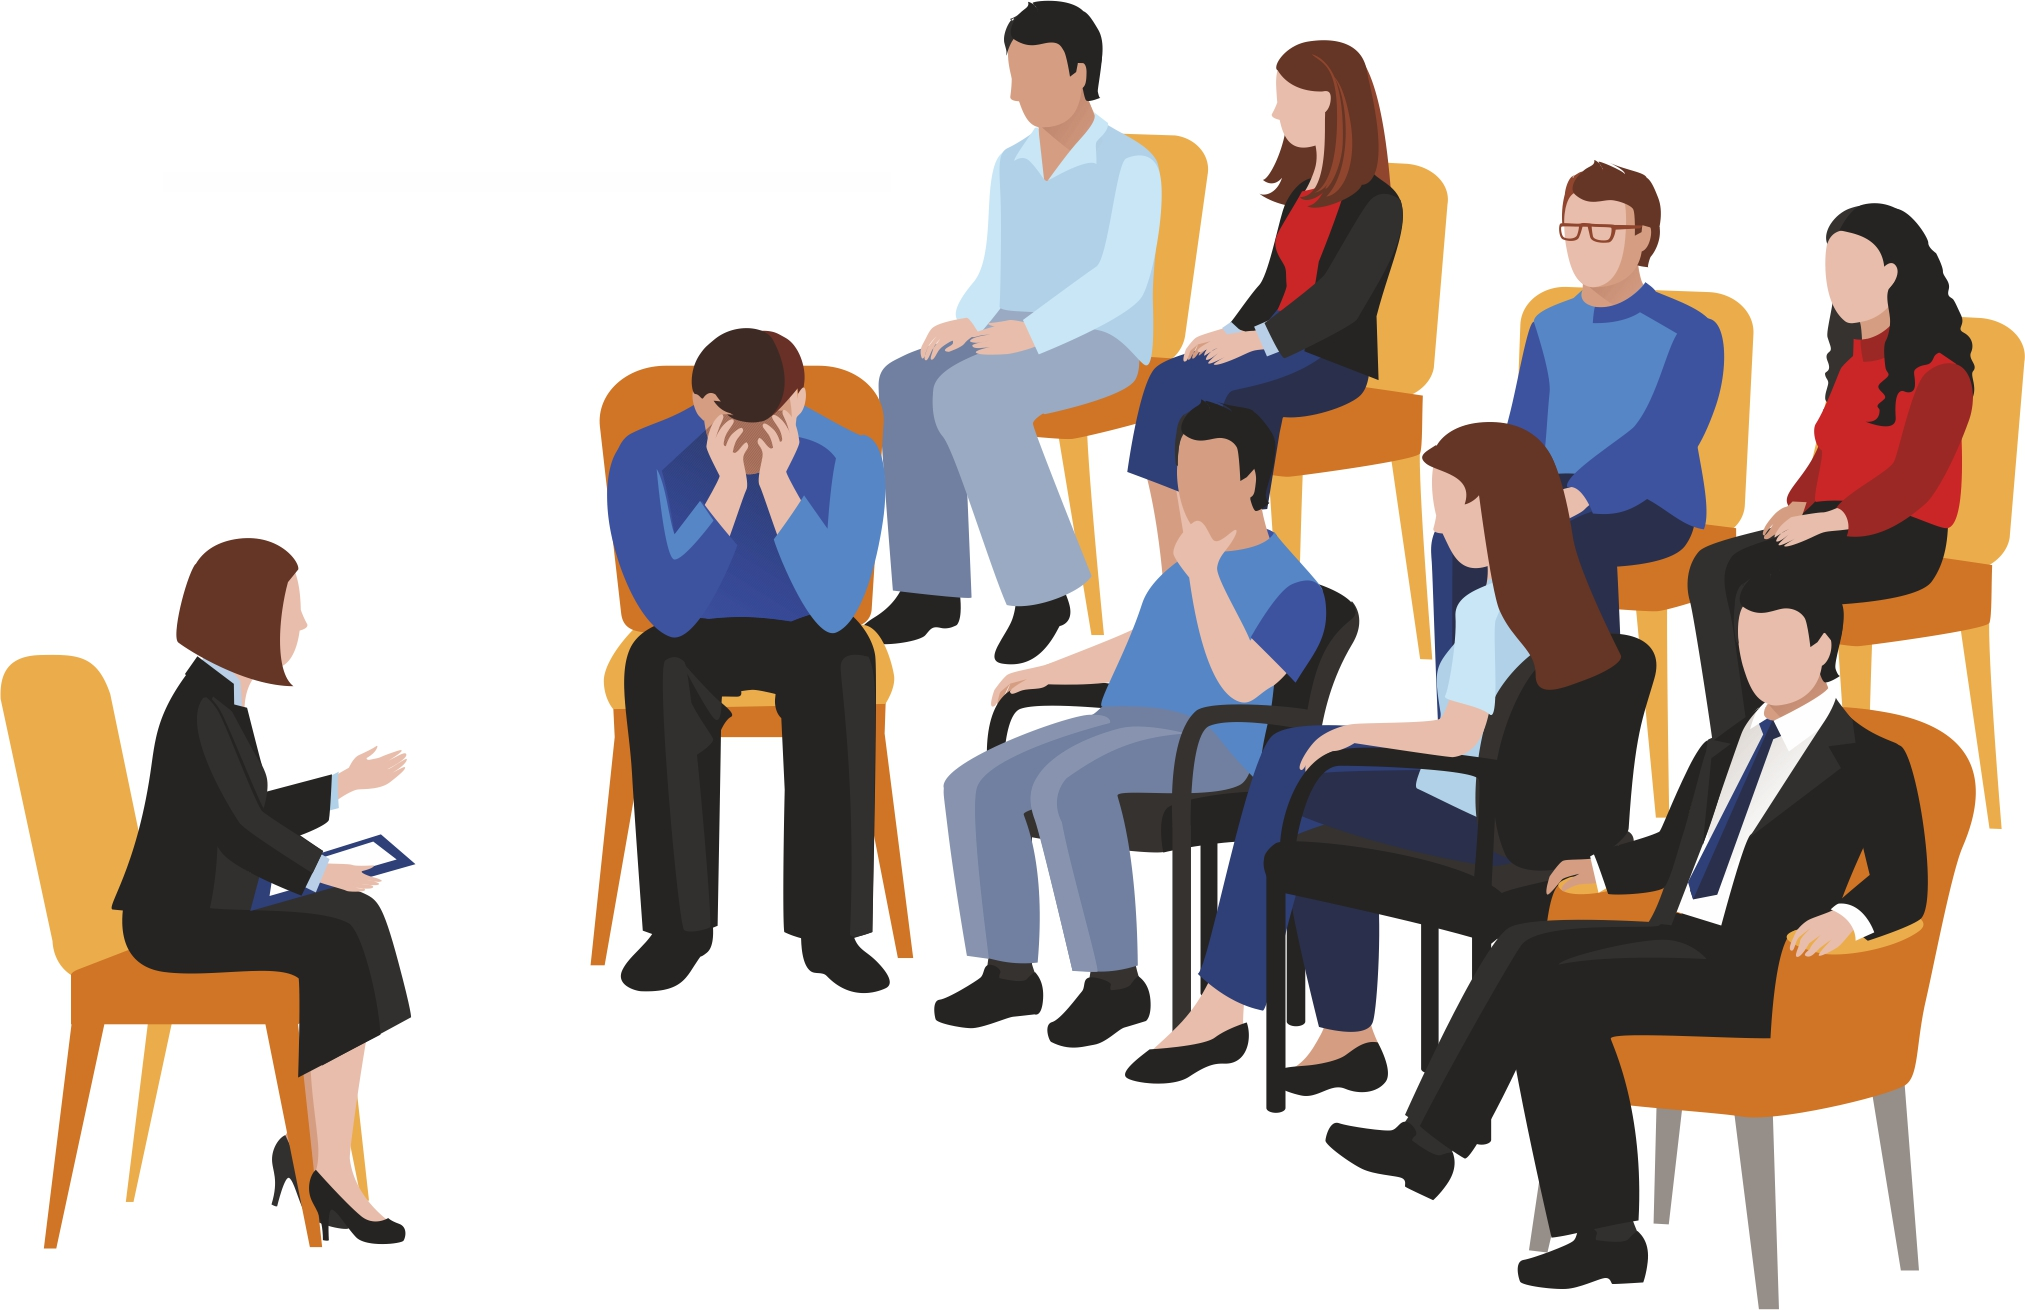
\includegraphics[scale = .5]{png/traditional.jpg}
            \end{figure}
        }
        \only<+>{
            \begin{itemize}
                \item surveys
                \item observational studies
                \item experiments
                \item case studies
                \item event sampling methodology (diaries)
                \item interviews
                \item meta-analysis
            \end{itemize}}
        \only<+>{
            \resizebox{\textwidth}{!}{
                \begin{tabular}{l | c | c | c | c | c | c }
                Id & Sex & Age & Condition & Variable A & Variable B & Variable C\\
                \hline \hline
                AAA & M & 24 & exp & 55:53 & 3 & apple\\
                AAB & F & 22 & exp & 53:47 & 2 & banana\\
                AAC & F & 28 & con & n/a   & 4 & banana\\
                AAD & M & 21 & con & 54:35 & 3 & banana
                \end{tabular}}
        }
\end{frame}

\begin{frame}
    \frametitle{Computational methods}
    \setbeamercovered{transparent}
    \begin{itemize}
        \item<1> extraction of unstructured data from external digital (i.e. web-based) sources
        \begin{itemize}
            \item<1> webscraping (extraction of data from existing webpages)
            \item<1> extracting data from web APIs (i.e. Twitter)
        \end{itemize}
        \item<1> analysis of textual data (natural language processing - NLP)
        \item<0> network and relational data analysis
        \item<0> working with big datasets (that do not fit into RAM of a single computer), in-database computations, distributed computing etc.
        \item<0> computer simulations
        \item<0> online experiments (A/B testing, experiments based on online games etc.)
    \end{itemize}
\end{frame}

\section[Data]{Data}

\subsection[Data Sources]{Data Sources}
\begin{frame}
    \setbeamercovered{transparent}
    \frametitle{Data Sources}
    \only<+>{
        \begin{figure}
            
\includegraphics[scale=.35]{png/data_everywhere.png}
        \end{figure}}
    \only<+>{
        \begin{figure}
            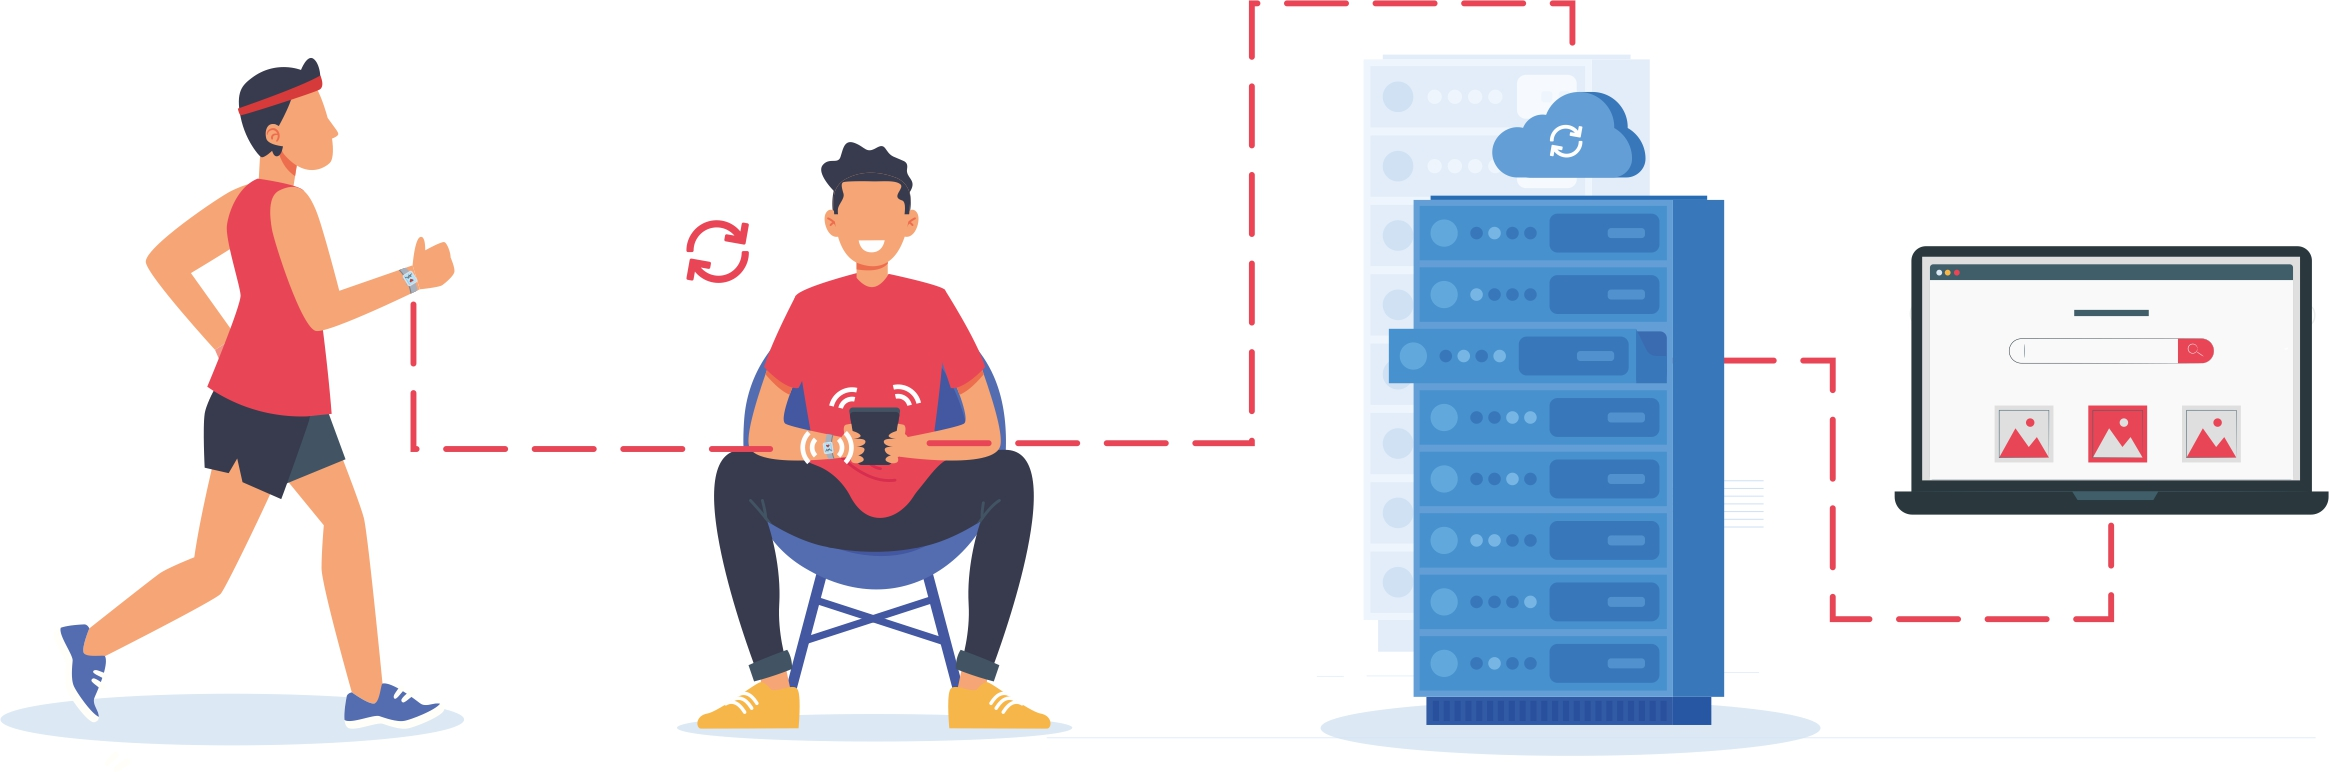
\includegraphics[scale = .5]{png/tracker.jpg}
        \end{figure}
    }
    \only<+>{
        \begin{itemize}
            \item<3> webpages
            \item<3> social media
            \item<0> smart devices
            \item<0> digital behavioral data
            \item<0> mobile phone networks
            \item<0> goverment data
            \item <0>...
        \end{itemize}
        \action<3>{\alert{The fact that you can get the data does not mean you should.}}
    }
\end{frame}

\subsection{Webscraping}

\begin{frame}
    \frametitle{Webscraping}
    \only<+>{
        \begin{figure}
            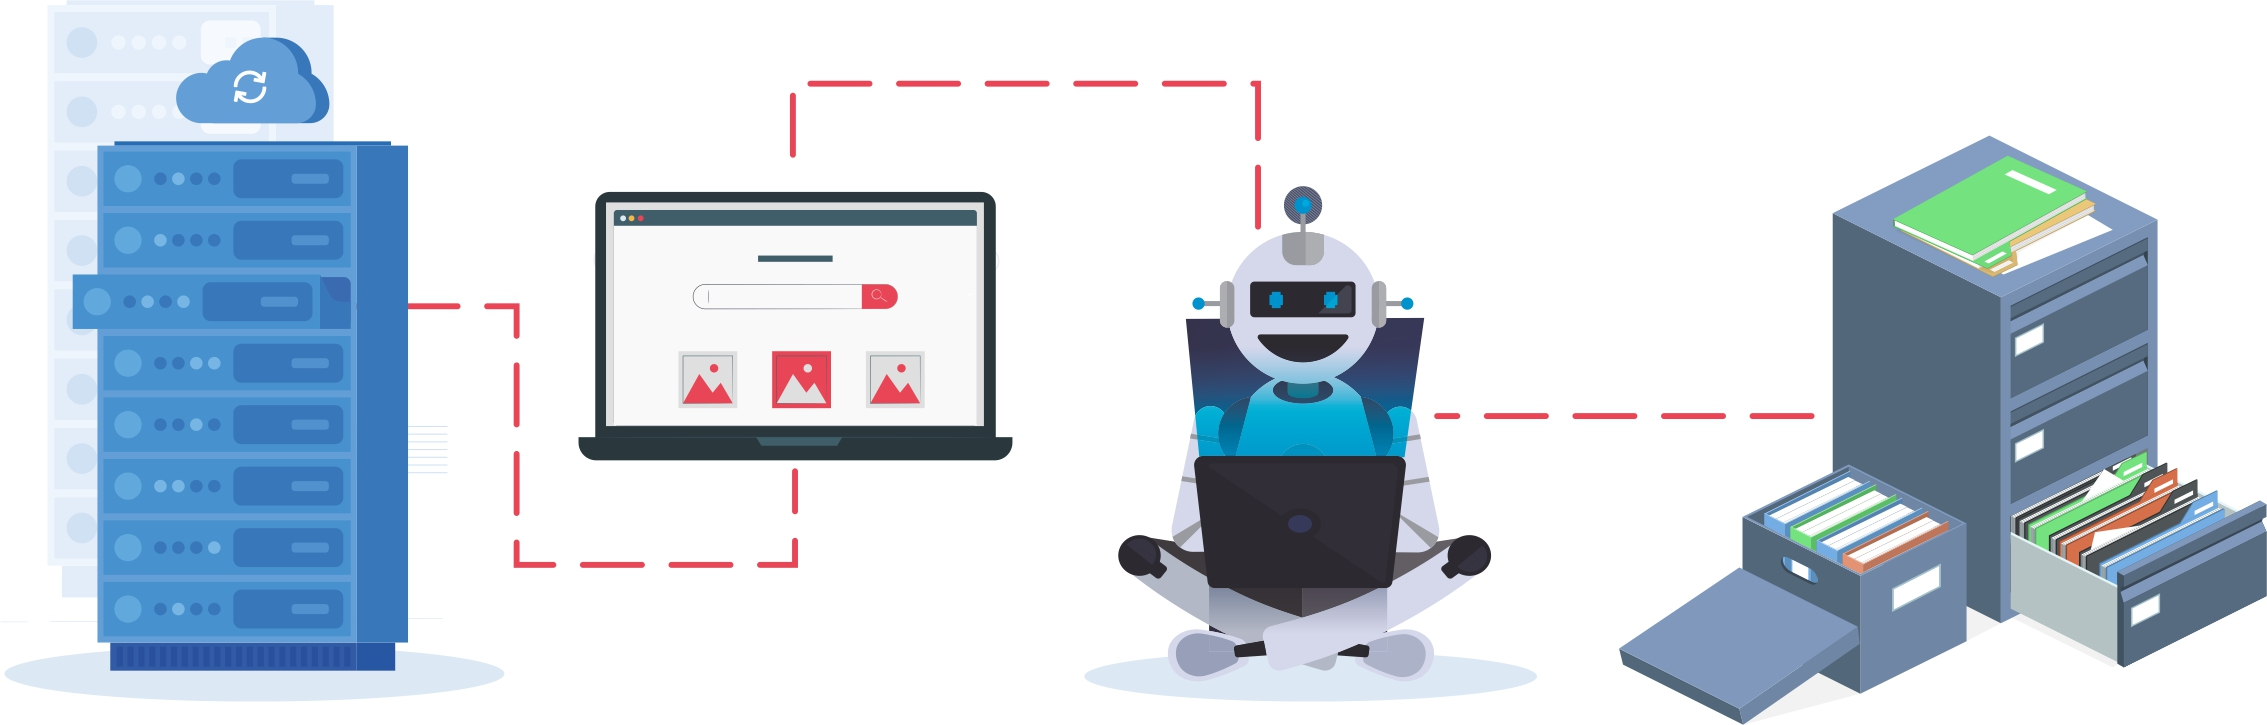
\includegraphics[scale = .5]{png/webscraping.jpg}
        \end{figure}
    }
    \only<+>{
        \begin{figure}
            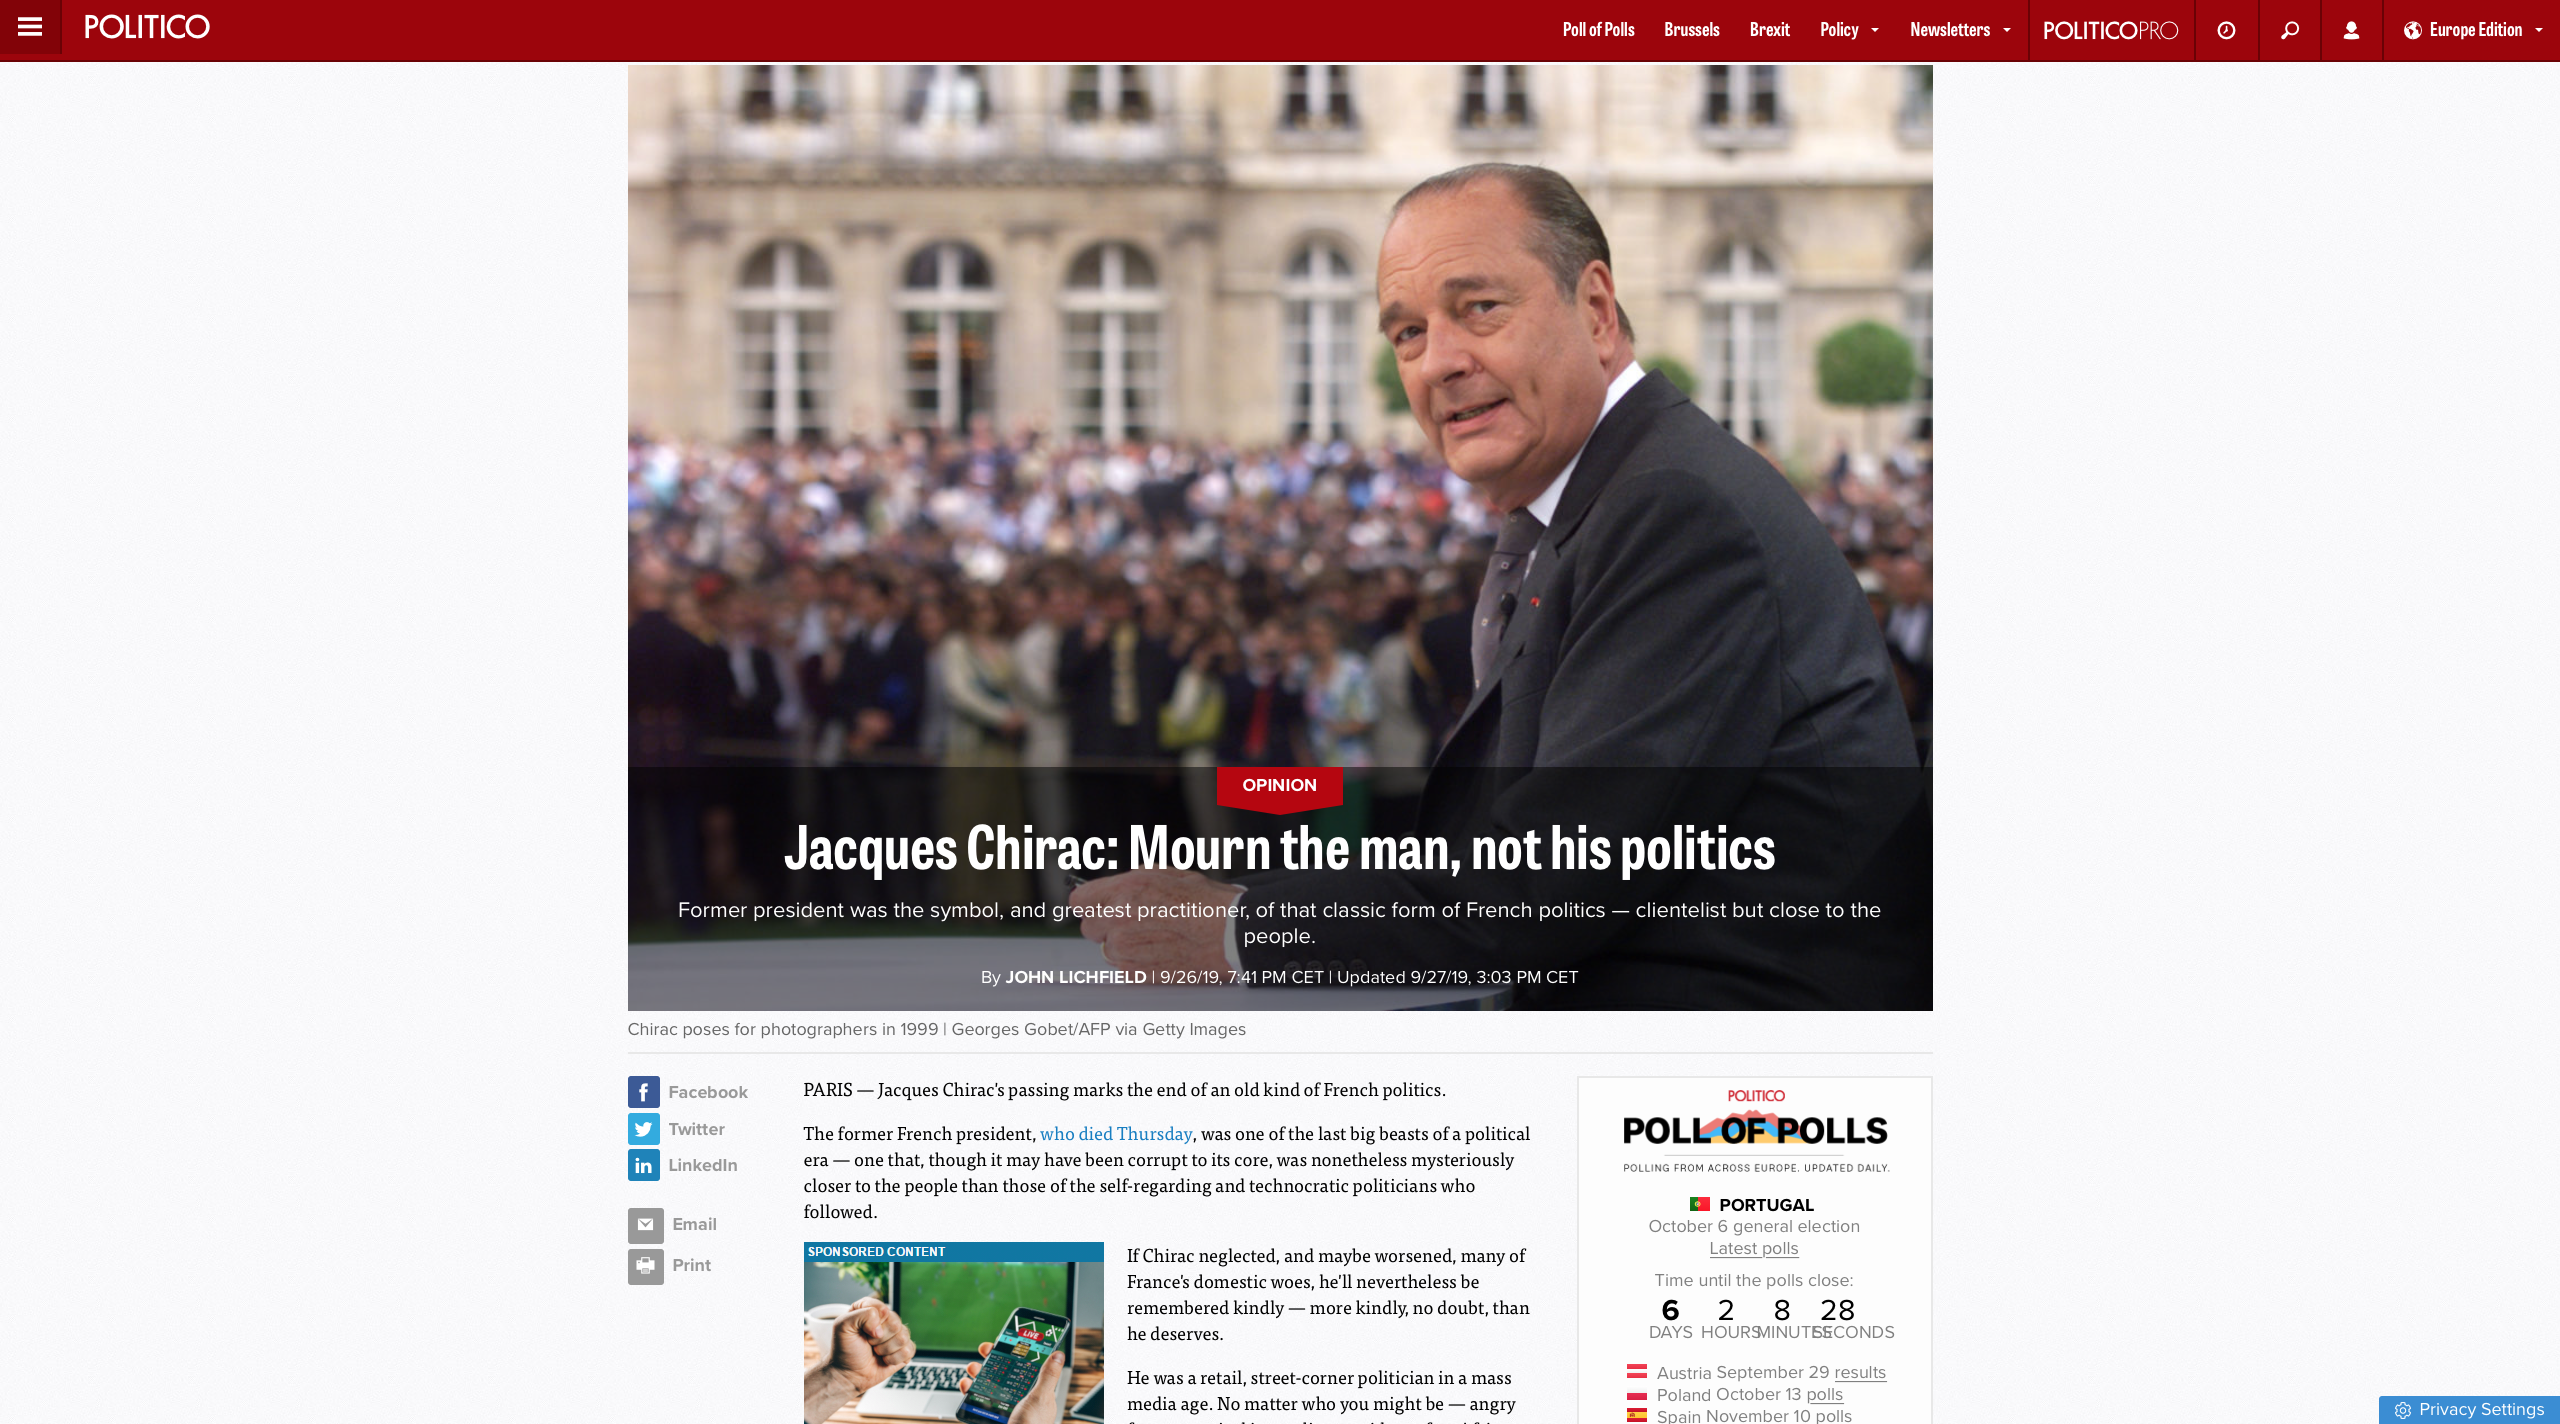
\includegraphics[scale = .22]{png/politico.png}
            \caption{from \textcolor{blue}{\href{https://www.politico.eu/article/jacques-chirac-mourn-the-man-not-his-politics/}{POLITICO Europe}}}
        \end{figure}
    }
    \only<+>{
        \begin{definition}
            \emph{Webscraping} is a process of (usually) automatic extraction of data from a website or multiple websites. In other words, it is a form copying the data from a website into a local database or spreadsheet.
        \end{definition}
    }
\end{frame}

\subsection{API}

\begin{frame}
    \frametitle{Application Programming Interface}
    \only<+>{
        \begin{figure}
            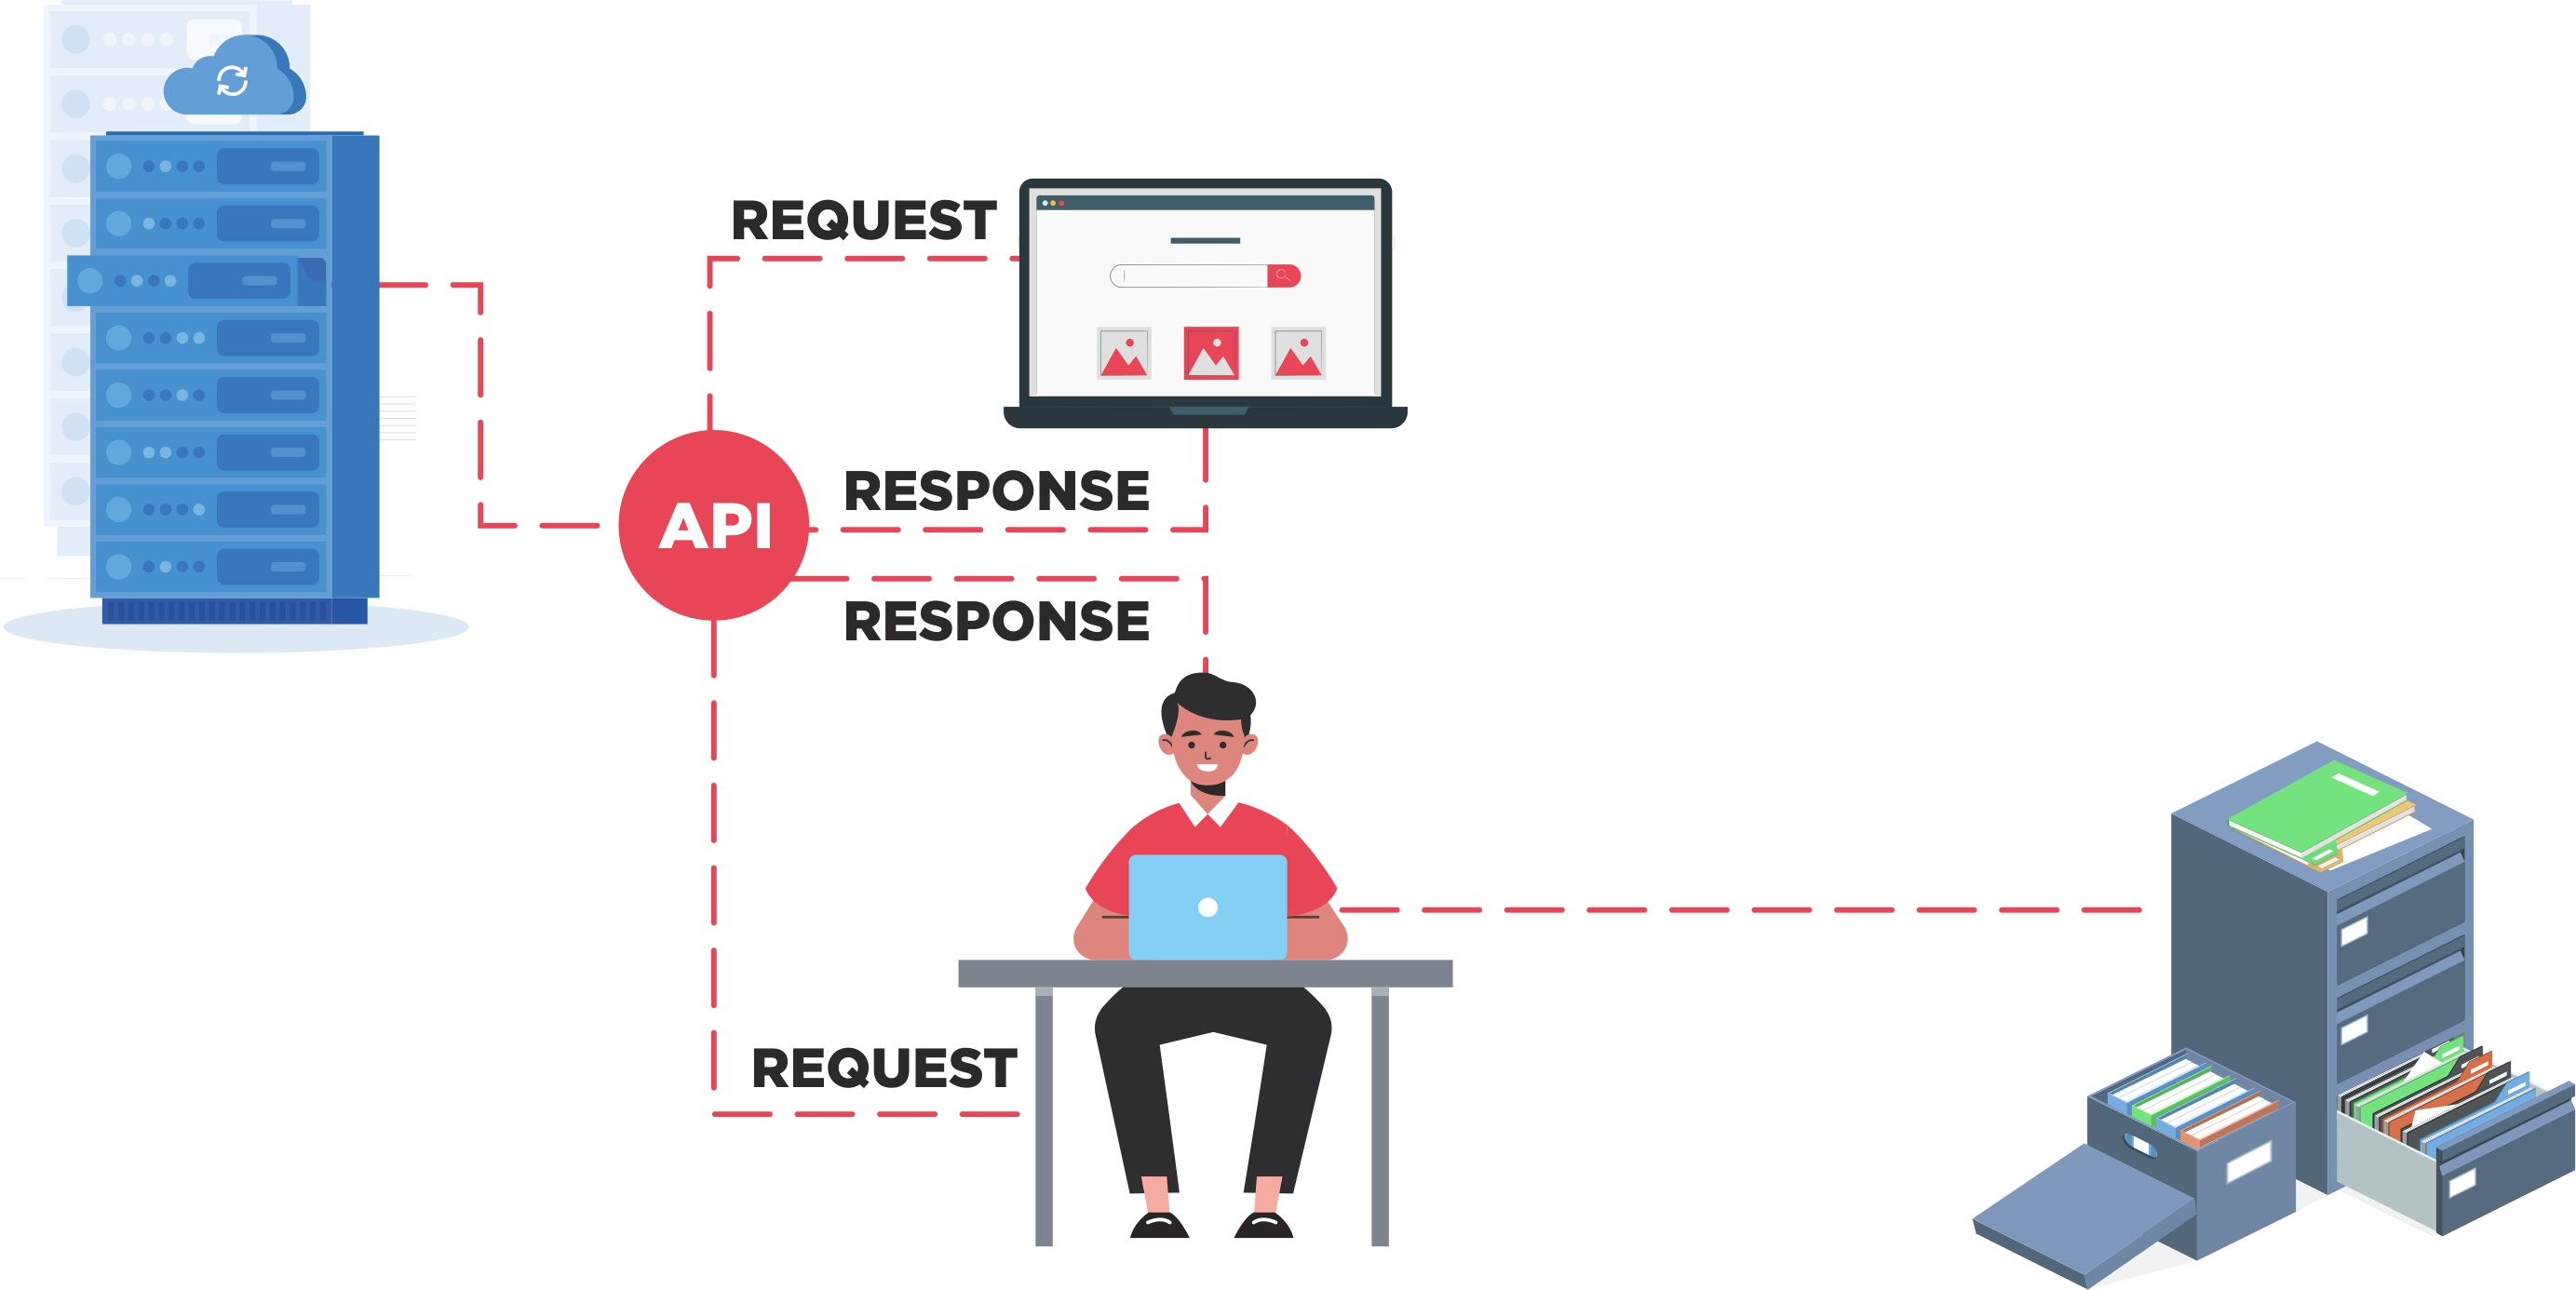
\includegraphics[scale = .4]{png/api.jpg}
        \end{figure}
    }
    \only<+>{
        \begin{figure}
            
\includegraphics[scale =.3]{png/twitter.png}
            \caption{from \textcolor{blue}{\href{https://developer.twitter.com/en/use-cases/analyze}{Developer Twitter}}}
        \end{figure}
    }
    \only<+>{
        \begin{definition}
            \emph{Aplication Programming Interface} is a communication protocol between a client and a server intended to simplify the building of client-side software. In other words, it is a contract between the client and the server which defines the format of possible requests and format of the response (i.e. format of the data).
        \end{definition}
    }
\end{frame}

\subsection[Data Formats]{Data Formats}

\begin{frame}
    \frametitle{Unstructured and Structured Data}
    \only<+>{
        \begin{figure}
            
\includegraphics[scale = .4]{png/structured.jpg}
        \end{figure}
    }
    \only<+>{\begin{columns}[t]
        \begin{column}{.5\textwidth}
            Unstructured Data:
            \begin{itemize}
                \item can't be displayed in rows and columns
                \item images, audio, video, e-mails, spreadsheets etc. (fun staff)
                \item requires more storage
                \item extremely hard to manage and analysis
            \end{itemize}
        \end{column}
        \begin{column}{.5\textwidth}
            Structured Data:
            \begin{itemize}
                \item can be displayed in rows and columns
                \item numbers, text, dates
                \item requires less storage
                \item easy to manage and analysis
            \end{itemize}
        \end{column}
        \end{columns}
    }
    \end{frame}
\begin{frame}
    \frametitle{Data Formats}
    \only<+>{
        Alice is a 17 years old young lady. Although her main field of interest is physics (especially quantum physics and string theory), she also fancies sport. Her favorite physical activities are fishing and football.
        Bob, on the other hand, is a naughty 15 years old boy who only loves literature, especially Szymborska poems touches his heart.
    }
    \only<+>{
        \textcolor{red}{Alice} is a \textcolor{blue}{17} years old young lady. Although her main field of interest is \underline{physics} (especially \textbf{quantum physics} and \textbf{string theory}), she also fancies \underline{sport}. Her favorite physical activities are \textbf{fishing} and \textbf{football}.
        \textcolor{red}{Bob}, on the other hand, is a naughty \textcolor{blue}{15} years old boy who only loves \underline{literature}, especially Szymborska \textbf{poems} touches his heart.
    }
    \only<+>{
        \resizebox{\textwidth}{!}{
            \begin{tabular}{l | c | c | c | c | c | c | c | c }
            Name & Sex & Age & Interest A & Interest A1 & Interest A2 & Interest B & Interest B1 & Interest B2\\
            \hline \hline
            Alice & F & 17 & physics & quantum physics & string theory & sport & fishing & football\\
            Bob & M & 15 & literature & poems & n/a & n/a & n/a & n/a \\
            \end{tabular}}

    }
\end{frame}

\begin{frame}[fragile]{JSON - JavaScript Object Notation}
\begin{minted}[fontsize=\footnotesize]{js}
{
    "name": "Alice",
    "age": 17,
    "interests": [
        {
            "name": "physics",
            "disciplines": [
                "quantum physics",
                "string theory"
            ]
        },
        {
            "name": "sport",
            "disciplines": [
                "fishing",
                "football"
            ]
        }
    ]
}
\end{minted}
\end{frame}

\begin{frame}[fragile]{JSON - JavaScript Object Notation}
\begin{minted}[fontsize=\footnotesize]{js}
{
    "name": "Bob",
    "age": 15,
    "interests": [
        {
            "name": "sport",
            "disciplines": [
                "football"
            ]
        }
    ]
}
\end{minted}
\end{frame}

\begin{frame}
    \frametitle{JSON - JavaScript Object Notation}
    \begin{definition}
        \emph{JavaScript Object Notation} is a lightweight text data format which is relatively easy to read for both human naked eye and computers. Although it derives from JavaScript it is a language-independent data format. JSON is built on two structures: a collection of key-item pairs and ordered list of values. JSON filenames use .json extension.
    \end{definition}
\end{frame}


\begin{frame}[fragile]{JSON Lines}
\begin{minted}[fontsize=\footnotesize]{js}
{"name":"Alice","age":17,"interests":[
    {"name":"physics","fields":["quantumphysics","stringtheory"]},
    {"name":"sport","fields":["fishing","football"]}
]}
{"name":"Bob","age":15,"interests":[
    {"name":"sport","disciplines":["football"]}
]}
\end{minted}
\begin{definition}
    \emph{JSON Lines} (newline-delimited JSON) is a lightweight text data format which can be processed one record at a time. Each line consists of a JSON. JSON Lines filenames use .jl or .jsonl extensions.
\end{definition}
\end{frame}

\section[NLP]{Natural Language Processing}

\begin{frame}
    \frametitle{Natural Language Processing}
    \only<+>{
        \begin{figure}
            
\includegraphics[scale = .7]{png/nlp.jpg}
        \end{figure}
    }
    \only<+>{
        \begin{definition}
            In general sense \emph{Natural Language Processing} (NLP) is an analytical approach which uses set of (usually) computer-based methods to extract meaning, topics or sentiment from natural language data (written or spoken). In other words, it is a set of computer algorithms which tries to synthesize human language.  \end{definition}
    }
    \only<+>{
        \begin{itemize}
            \item tokenization
            \item stemming
            \item lemmatization
            \item sentiment analysis
            \item vector models
            \item topic modeling
            \item part of speech tagging
            \item entities analysis
    \end{itemize}
    }

\end{frame}

\begin{frame}
    \frametitle{Semantic Space}
    \only<+>{
        \begin{figure}
            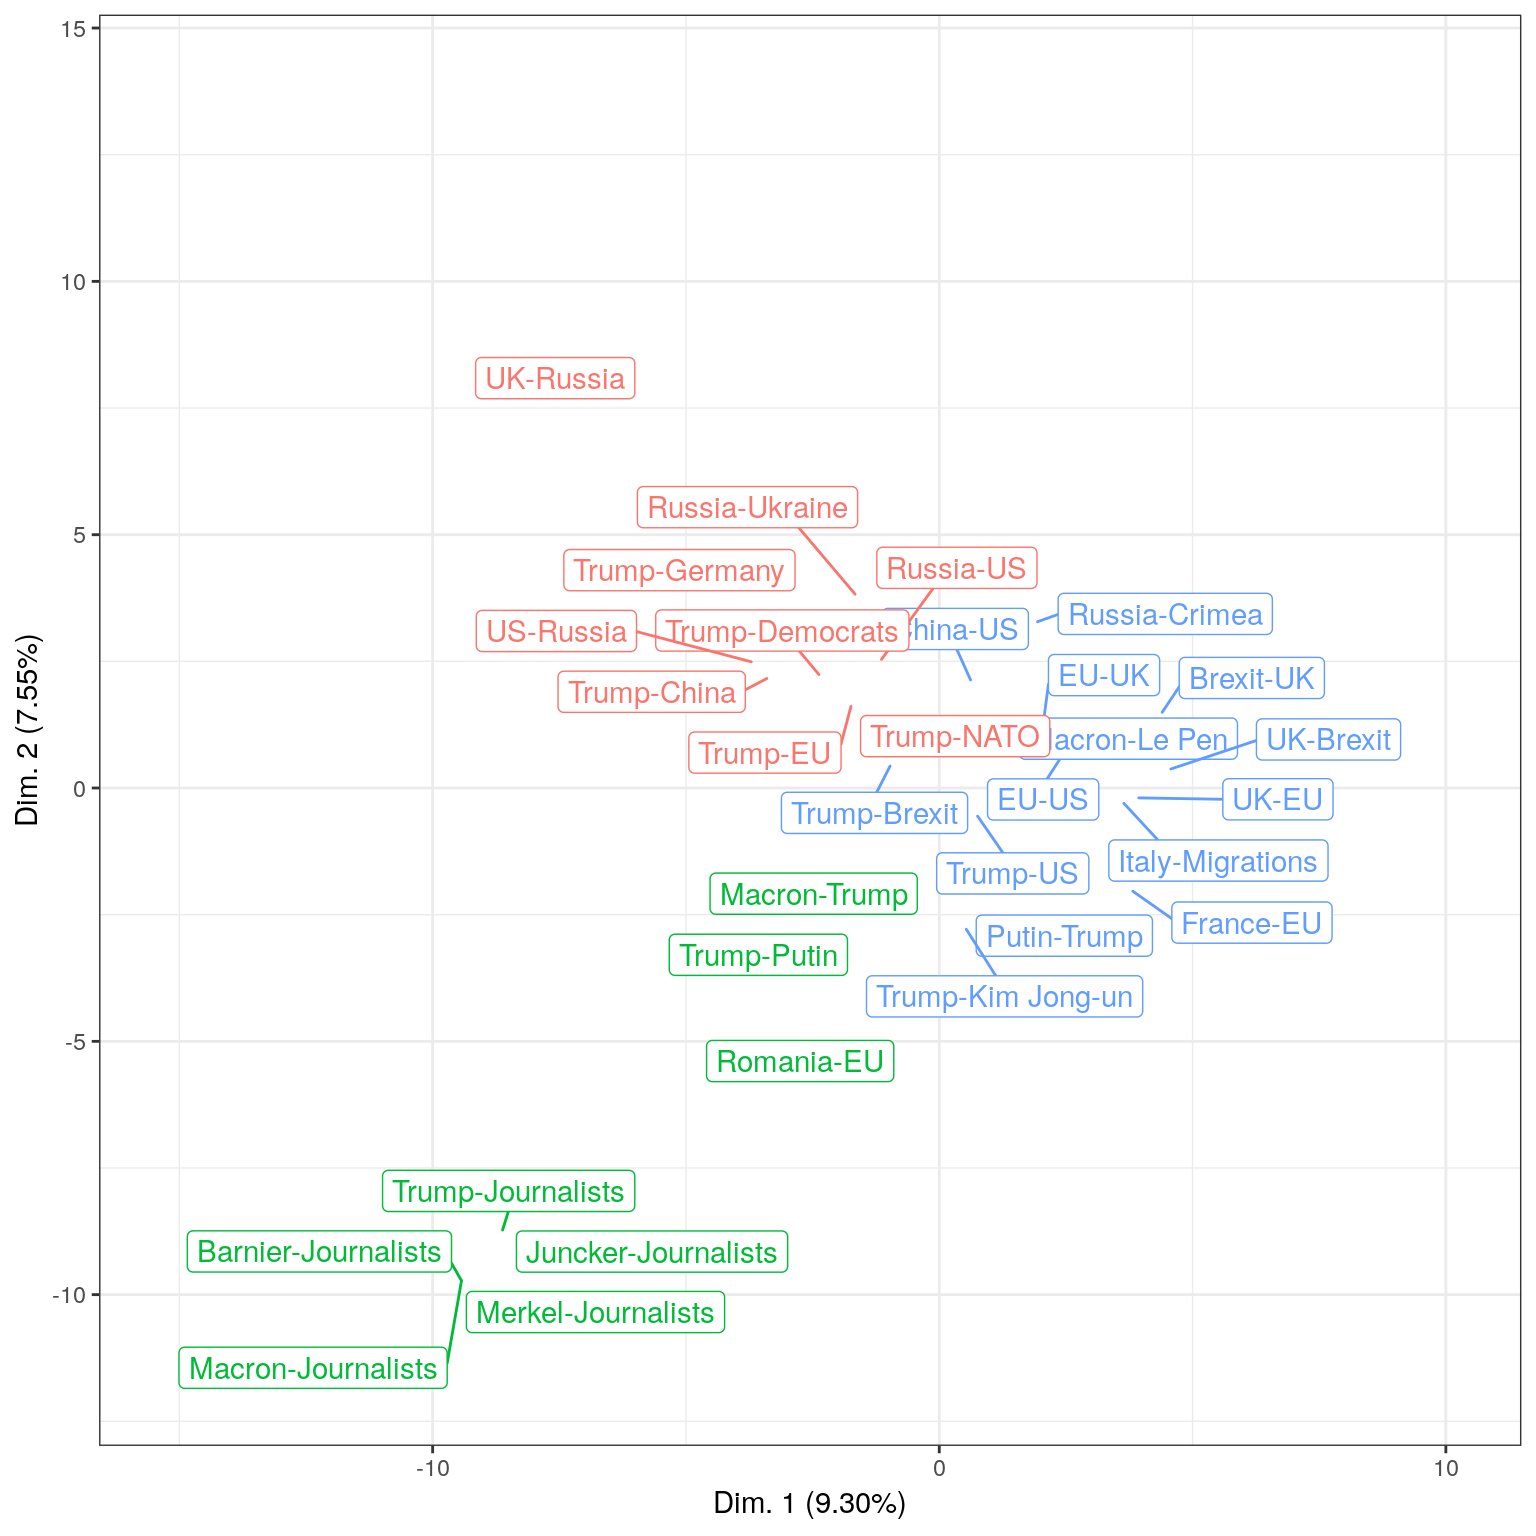
\includegraphics[scale = .4]{png/semantic_space-1.png}
        \end{figure}
    }
    \only<+>{
        \begin{figure}
            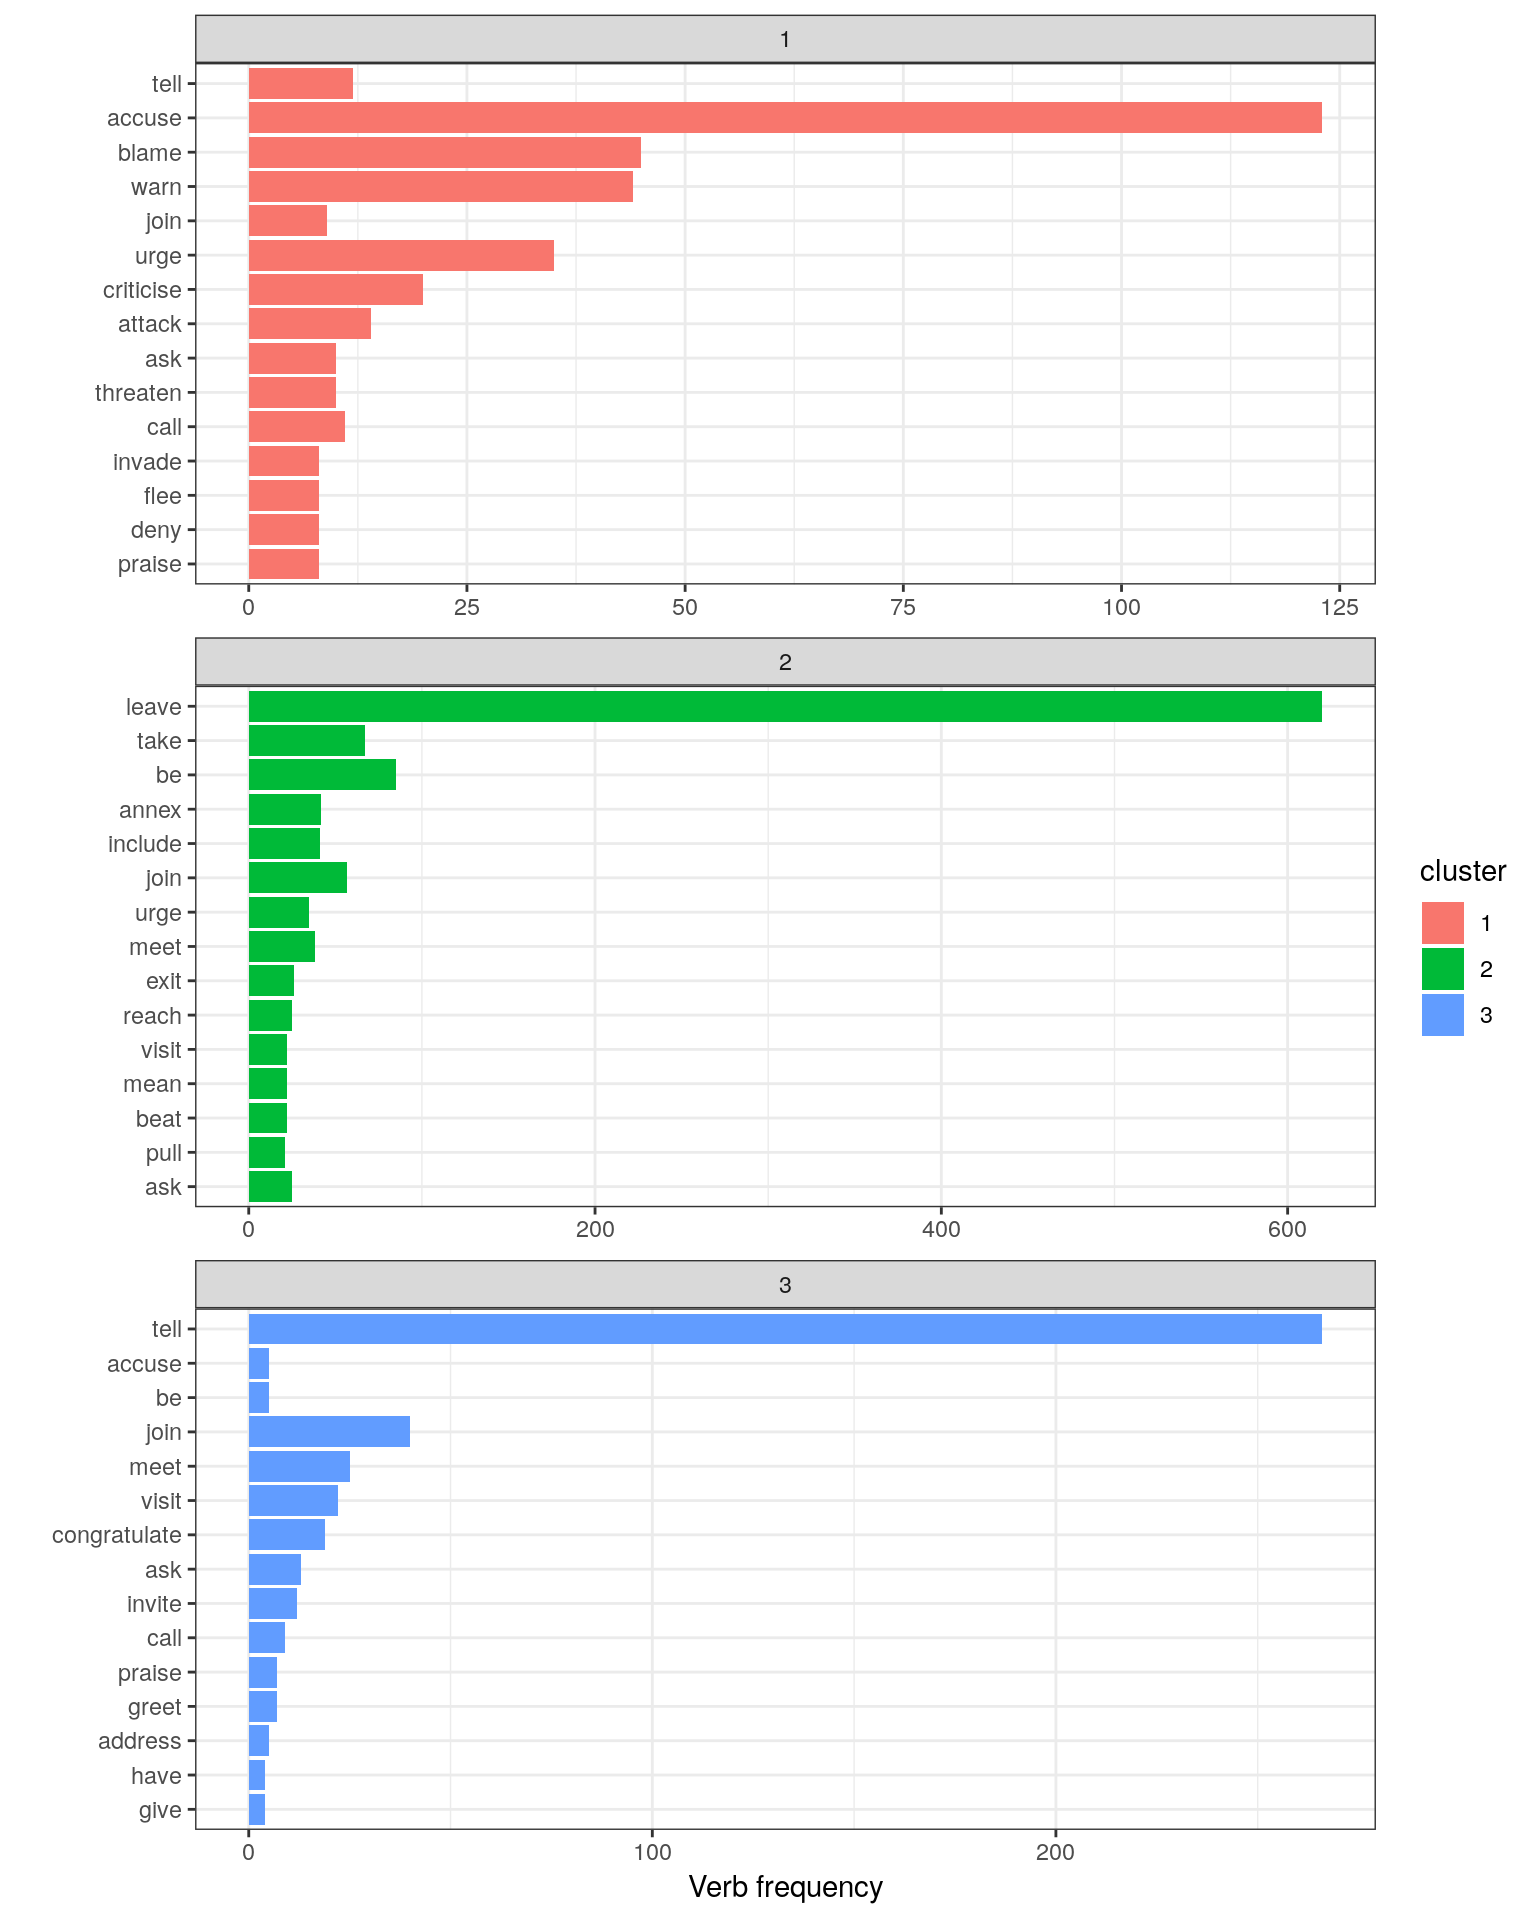
\includegraphics[scale = .3]{png/semantic_clusters_words-1.png}
        \end{figure}
    }
\end{frame}

%%% LITERATURE %%%%%%%%%%%%%%%%%%%%%%%%%%%%%%%%%%%%%%%%%%%%%%%%%%%%%%%%%%%%%%%%
\begin{frame}
    \frametitle{Literature to read}
    \nocite{*}
    \AtNextBibliography{\footnotesize}
    \printbibliography[title=Literature]
\end{frame}

\end{document}
